\documentclass[11pt,a4paper]{article}
\usepackage[T1]{fontenc}
\usepackage[utf8]{inputenc}
\usepackage{lmodern,microtype}
\usepackage[margin=27mm]{geometry}
\usepackage{amsmath,amssymb,amsthm,mathtools}
\usepackage{graphicx,booktabs,tabularx,array,multirow}
\usepackage{float}
\usepackage{algorithm,algpseudocode}
\usepackage{enumitem,xcolor,tikz}
\usetikzlibrary{arrows.meta,positioning}
\usepackage{listings}
\usepackage[hyphens]{url}
\usepackage{xurl}
\usepackage[colorlinks=true,linkcolor=blue!45!black,citecolor=blue!45!black,urlcolor=blue!45!black]{hyperref}
\usepackage[capitalise,noabbrev]{cleveref}
\usepackage{fancyhdr}
\pagestyle{fancy}\fancyhf{}
\fancyhead[L]{\small ECC2K-130 walks on Blackwell GPUs}
\fancyhead[R]{\small Adam Buran}
\fancyfoot[C]{\thepage}
\setlength{\headheight}{14pt}
\setlength{\emergencystretch}{2em}
\setlist{nosep,leftmargin=*}
\newcommand{\F}{\mathbb{F}}
\newcommand{\HW}{\operatorname{HW}}
\newcommand{\spread}{\operatorname{spread}}
\newcommand{\xor}{\mathbin{\oplus}}
\newcommand{\code}[1]{\texttt{\small #1}}
\newcommand{\Bps}{\text{ billion updates/s}}
\newcolumntype{Y}{>{\raggedright\arraybackslash}X}
\newcommand{\hashval}[2]{\texttt{\footnotesize #1}\newline\texttt{\footnotesize #2}}
\renewcommand{\arraystretch}{1.08}
\newtheorem{proposition}{Proposition}
\lstset{basicstyle=\ttfamily\footnotesize,breaklines=true,columns=fullflexible,
  keepspaces=true,frame=single,rulecolor=\color{black!20},xleftmargin=0.5em,xrightmargin=0.5em}
\hypersetup{pdftitle={High-Throughput ECC2K-130 Walks on Blackwell GPUs},pdfauthor={Adam Buran},
  pdfsubject={Packed binary-field arithmetic and cooperative batch inversion}}

\title{\textbf{High-Throughput ECC2K-130 Walks\\on Blackwell GPUs}\\[0.45em]
  \large Packed Binary-Field Arithmetic and Cooperative Batch Inversion}
\author{Adam Buran}
\date{September 21, 2026\\[0.2em]\small Research preprint draft}

\begin{document}
\maketitle
\begin{abstract}
Efficient elliptic-curve collision-search implementations require a joint treatment of finite-field arithmetic, walk semantics, and the GPU memory hierarchy. We describe an implementation for the public ECC2K-130 parameters over $\F_{2^{131}}$ using packed polynomial coordinates, native carryless multiplication, an eight-branch table walk, and cooperative inversion across groups of four warps. The last arithmetic refinement reduces a polynomial square in compressed even and odd coefficient streams before interleaving the result. Together with a rotated four-warp inversion tree, explicit non-aliasing buffers, compact metadata, and a 640-thread block geometry, the accepted configuration reaches a median of \textbf{22.100934 billion scheduled scalar-slot updates per second} on one NVIDIA RTX PRO 6000 Blackwell Server Edition. Five confirmation runs each execute 504,658,657,280 updates; their range is 22.089525--22.166455 billion updates/s. The median improvement over an alternating, same-device baseline is \textbf{11.32\%}; every candidate sample exceeds every baseline sample. Screening runs attribute most of that gain to the inversion tree at the wider geometry and three to four percentage points to the square, but the components were not isolated in a controlled ablation. A separate distinguished-point collection run reaches \textbf{21.548499 billion updates/s} and produces 12,387 records with zero reported drops. Independent arithmetic probes, 300 reference trail replays, equal complete report corpora, and bidirectional checkpoint continuation support the implementation evidence. We distinguish these results from effective collision-search throughput: history-dependent cycle avoidance, exceptional affine inputs, and long-run collision statistics remain outside the accepted performance claim. The work establishes a reproducible GPU implementation result, without asserting a completed ECC2K-130 solution or a new asymptotic discrete-logarithm algorithm.
\end{abstract}
\noindent\textbf{Keywords:} ECC2K-130; Koblitz curves; GPU cryptanalysis; binary fields; batch inversion; carryless multiplication; reproducible benchmarking.

\section{Introduction}
The ECC2K-130 challenge provides a concrete setting in which to study the cost of elliptic-curve computation over a binary field. Its arithmetic is especially suitable for low-level optimization: field addition is XOR, the Frobenius endomorphism is linear, and many independent walks can share inversions. These features also create a difficult implementation tradeoff. A larger batch saves inversions but increases the working set; more parallel work can hide latency but consumes registers and shared memory; a cheaper iteration function can change the statistical behavior on which collision search depends.

This paper studies the current accepted high-throughput research configuration in the project's archived ECC2K-130 implementation, identified as \code{warps4\_poly\_compact640}. The source and measurement receipt are fixed by content hashes. The result is a complete walk-loop measurement on one GPU, including selection and coordinate updates, rather than an isolated multiplication benchmark. Its central finding is that arithmetic specialization and scheduling must be designed together. Cooperative inversion alone was not sufficient in earlier experiments; the accepted combination uses a rotated product tree, compact live metadata, restricted pointers, and a specialized polynomial square.

The contributions are:
\begin{enumerate}
\item A precise description of the eight-branch, automorphism-aware table walk and of the history that its short-cycle rule adds to the state.
\item A two-level inversion schedule whose multiplication budget is $5+5/(BW)$ per ordinary affine update, with $B=16$ slots per thread and $W=4$ collaborating warps.
\item An exact even/odd-stream square-and-reduce map for the internal degree-131 polynomial representation, accompanied by a reproducible basis-vector identity check.
\item An evidence-backed evaluation of a 22.100934-billion-update/s configuration, including all five confirmation samples, a configuration-by-configuration comparison with the baseline, the screening sequence that led to it, resource usage, collection performance, and validation limits.
\item First-order estimates for the walk's open questions: the unreachable part of the selector domain, the probability of an exceptional addition, merge coalescence under the history rule, and the frequency of six-step fruitless cycles.
\end{enumerate}

The measured implementation is the strongest accepted configuration in the evidence set examined here. We use \emph{state of the art} only as a research objective and literature context: a global fastest-solver claim would additionally require a current, comparable survey and validated collision efficiency for this particular walk. The archived result does not supply either a completed challenge solution or that full comparison.

\section{Background and comparison scope}
Pollard's rho method provides the classical low-memory approach to generic discrete logarithms~\cite{pollard1978}. Distinguished-point methods permit many processors to contribute trails to a common collision search~\cite{vow1999}. In that setting, iteration speed is only one component of performance: trail coalescence, fruitless cycles, endpoint production, replay, and collision usefulness all affect the work needed for a successful computation.

The ECC2K-130 work of Bailey et al. exploits Frobenius and negation symmetries and analyzes a specific iteration function~\cite{bailey2009}. Bernstein et al. subsequently report more than 63 million iterations/s on a GTX 295 graphics card, using bitsliced arithmetic and carefully managed GPU storage~\cite{bernstein2012}. Bos et al. report 25.57 million iterations/s across the six usable SPUs of a PlayStation 3~\cite{bos2010}. These are valuable historical reference points, but the hardware, arithmetic representation, and iteration function differ from the present table-walk implementation.

Batch inversion and normal-basis exponentiation are established techniques~\cite{montgomery1987,itoh1988}. Likewise, the difficulty of exploiting automorphisms without introducing fruitless cycles is a known issue~\cite{negation2011}. Our contribution is a concrete implementation and its measured combination of optimizations. We do not claim to introduce Pollard rho, the use of Frobenius orbits, table walks in general, or the batch-inversion principle.

\begin{table}[t]
\centering\small
\begin{tabularx}{\linewidth}{@{}lYrl@{}}
\toprule
Work & Hardware / scope & Rate & Unit\\
\midrule
Bos et al.~\cite{bos2010} & Cell, six SPUs; historical walk & 25.57 & million/s\\
Bernstein et al.~\cite{bernstein2012} & GTX 295 card; historical walk & $>63$ & million/s\\
Local control & One RTX PRO 6000; table walk & 19.852741 & billion/s\\
This configuration & Same GPU; same table walk & 22.100934 & billion/s\\
Collection mode & Same candidate; DP weight 34 & 21.548499 & billion/s\\
\bottomrule
\end{tabularx}
\caption{Contextual throughput comparison. The first two rows are published historical iteration rates. The last three use the scheduled-slot metric in \cref{sec:methodology}. Only the two local benchmark rows constitute a direct implementation comparison; the collection row is a single separate run.}
\label{tab:context}
\end{table}

\section{Curve, representations, and walk semantics}
\subsection{Curve and field}
The implemented curve is
\begin{equation}
 E:\quad y^2+xy=x^3+1\qquad\text{over }\F_{2^{131}},
\end{equation}
with the prime-order subgroup parameter recorded in the generated source as
\begin{equation}
 \ell=680564733841876926932320129493409985129.
\end{equation}
For an affine point $R=(x,y)$, negation is $-R=(x,y+x)$ and Frobenius is $\sigma(R)=(x^2,y^2)$. The ordinary automorphism orbit is $\{\pm\sigma^k(R):0\leq k<131\}$, of size at most 262. Orbit arithmetic and exceptional orbit sizes must be distinguished from a heuristic uniform random map on $\ell/262$ objects.

The code uses a permuted type-II optimal normal basis indexed by $e\in\{1,\ldots,131\}$, with $263=2\cdot131+1$ and the index operation
\begin{equation}
 \operatorname{fold}(u)=\min(u\bmod263,\;263-(u\bmod263)).
\end{equation}
Squaring maps index $e$ to $\operatorname{fold}(2e)$. A normal-basis coordinate vector is useful for Hamming weight and walk selection. Persistent coordinates and most multiplication intermediates instead use an internal polynomial basis; conversion is an exact generated linear map.

The internal reduction polynomial is represented by the bit string
\begin{equation}\label{eq:modulus}
 F=\mathtt{0xD1D0D000D0000000D000000000000000D}.
\end{equation}
Equivalently, with the bit in position $i$ denoting the coefficient of $z^i$,
\begin{equation}
 F(z)=z^{124}+(1+z^2+z^3)(1+z^{64}+z^{96}+z^{112}+z^{120}+z^{128}).
\end{equation}
This internal representation is distinct from the sparse polynomial $z^{131}+z^{13}+z^2+z+1$ also listed by the parameter generator, and the choice is structural. Let $\zeta$ be a primitive 263rd root of unity and $\beta=\zeta+\zeta^{-1}$, so that the normal-basis elements are $\beta_e=\zeta^e+\zeta^{-e}$. The minimal polynomial of $\beta$ over $\F_2$ is produced by the recurrence
\begin{equation}\label{eq:recurrence}
 f_0=1,\qquad f_1=z+1,\qquad f_{j+1}=z f_j+f_{j-1},
\end{equation}
and a direct computation confirms $f_{131}=F$ exactly. The internal polynomial basis is therefore $1,\beta,\ldots,\beta^{130}$: the same element $\beta$ generates both representations. Since
\begin{equation}
 \beta^j=\sum_{0\leq i<j/2}\binom{j}{i}\beta_{j-2i}\quad\text{in characteristic two},
\end{equation}
the change of basis is a fixed and highly structured linear map, closely related to the type-II optimal polynomial bases of Bernstein and Lange~\cite{bernstein2010opb}. This is what makes it affordable to keep persistent state in polynomial form while still evaluating the normal-basis weight and selector on every step.

The price is a denser modulus: $F$ has 19 terms where the pentanomial has five. The factored form above limits that cost, because reduction applies only the three-term factor $1+z^2+z^3$ at six byte-aligned offsets, together with the single term $z^{124}$. With the pentanomial, the selector would instead need an unstructured $131\times131$ basis change on every step. That alternative was not measured, so the tradeoff is offered as the design rationale and not as a measured optimum. The square circuit below is tied to \cref{eq:modulus}; substituting another representation without changing the linear maps would be incorrect.

\subsection{Eight-branch table selection}
Let $P,Q$ be the public challenge points. The reference implementation deterministically constructs $H=8$ table points $T_h=[a_h]P+[b_h]Q$, along with all $\sigma^k(T_h)$. The coefficients are fixed by a public branch-index seed and modular reduction; they are part of the walk identity. The device reads the table coordinates in polynomial representation.

Write the normal-basis $x$ coordinate as $(x_e)$. Define $L$ by
\begin{equation}
 L(\operatorname{fold}(2^t))=t,\qquad 0\leq t<131.
\end{equation}
For $w=\sum_e x_e$ with $w\not\equiv0\pmod{131}$, the raw selection is
\begin{align}
 h(R)&=\lfloor w/2\rfloor\bmod8,\\
 k(R)&=w^{-1}\sum_e L(e)x_e\pmod{131},\\
 p(R)&=\underset{e:x_e=1}{\arg\max}\;((L(e)-k(R))\bmod131),\\
 \epsilon(R)&=y_{p(R)}.
\end{align}
Before the cycle correction, the update is
\begin{equation}\label{eq:walk}
 f(R)=R+(-1)^{\epsilon(R)}\sigma^{k(R)}(T_{h(R)}).
\end{equation}
Only the selected normal-basis coordinate of $y$ is needed: a precomputed linear row evaluates it from polynomial $y$, avoiding a full conversion. The $x$ conversion is retained for the selector and distinguished-point test.

\begin{proposition}[Raw-selector equivariance]
On the domain where the selector and affine update are defined, the raw map in \cref{eq:walk} satisfies $f(\sigma R)=\sigma f(R)$ and $f(-R)=-f(R)$.
\end{proposition}
\begin{proof}
Squaring permutes the support and adds one to every $L(e)$ modulo 131. The weight is unchanged, so $k$ increases by one and the cyclic ordering defining the pivot is preserved. The selected $y$ bit is carried along with its pivot, making $\epsilon$ Frobenius-invariant. Under negation $x$ does not change, while $y$ becomes $y+x$. The pivot lies in the support of $x$, hence its $y$ bit flips. Applying these transformations to the chosen addend gives the two identities.
\end{proof}

The statement has an explicit domain: a zero coordinate has no pivot, and weights divisible by 131 do not admit the displayed inverse. Inside the prime-order subgroup this part of the domain is never left. Every subgroup point is a double, so $\operatorname{Tr}(x)=\operatorname{Tr}(a_2)=0$ for this curve, whose $x^2$ coefficient $a_2$ is zero. Each element of the normal basis has trace one, hence $\operatorname{Tr}(x)\equiv w\pmod2$ and the weight $w$ is always even. This is also why the branch index uses $\lfloor w/2\rfloor$. Since $0\leq w\leq131$ and 131 is odd, $w\equiv0\pmod{131}$ forces $w=0$, that is $x=0$. The only affine point with $x=0$ is $(0,1)$, which has order two and does not lie in the subgroup of order $\ell$. The selector is therefore defined at every point a trail can reach. The remaining exceptional case is the affine addition itself, which is treated in \cref{sec:exceptional}.

\subsection{History-dependent cycle avoidance}\label{sec:history}
The actual implementation augments the point with the three most recent step tags. A tag is $(h,k,\epsilon)$, packed into a 16-bit value. If the proposed tag is the sign-opposite of the preceding tag, it would immediately undo that addition. The code also rejects the four-step pattern where the new tag cancels the second previous tag and the most recent tag cancels the third previous tag. It increments $h$ modulo eight until the test clears, then updates history.

At most two branch values can be prohibited by these two equality tests for a fixed $(k,\epsilon)$, so the branch scan terminates for eight branches. The rule removes those particular algebraic cancellation patterns. It neither enumerates all possible cycles nor proves a random-map collision constant.

Most significantly, the resulting transition is a function of \emph{point and history}. Two trails at the same point can select different successors when their histories differ. Equivariance extends to consistently transformed histories, but it does not by itself prove that projected point collisions coalesce as in a point-only rho walk.

A first-order estimate shows that the effect on coalescence is small. Write $r=2\cdot8\cdot131=2{,}096$ for the number of signed addends, and model the raw tag as uniform and independent of the history. When two trails meet at a point, both propose the same raw tag $t$. The correction changes the successor of a trail only if $t$ cancels that trail's most recent tag, which has probability about $1/r$, or completes the four-step pattern, which has probability about $1/r^2$. The two trails therefore take different successors at the meeting point with probability about $2/r\approx9.5\times10^{-4}$. After one shared step their most recent tags agree, so the two-step test agrees; after three shared steps the three stored tags agree and the trails are identical from then on. In this model roughly $0.1\%$ of merges fail to coalesce, which is negligible against the other constants of the search.

Longer fruitless cycles are not negligible by the same argument. A six-step cycle $a,b,c$ followed by $-a,-b,-c$ in some order survives the two rules for three of the six orders, and a trail that enters it repeats it indefinitely. In the same model the probability per step is about $3/r^3\approx3.3\times10^{-10}$. A DP34 trail has mean length $2^{25.27}\approx4.0\times10^{7}$ steps (\cref{sec:dp}), so on the order of $1\%$ of trails would enter a six-step cycle before reaching a distinguished point; cycles of length eight and more are rarer by further factors of $r$. The client has a guard for this case: \code{--max-iters} restarts any walk that exceeds a step limit, checked every 4,096 steps. The guard is disabled by default and was not enabled in the measured commands. If the estimate is right, the limit matters, because a trapped trail consumes the whole limit: at the customary limit of 20 mean trail lengths~\cite{vow1999}, a $1\%$ trapped fraction would cost between a sixth and a fifth of all work. These figures are heuristic and come from the uniform model above, following the analysis style of Bernstein, Lange, and Schwabe~\cite{negation2011}. They have not been measured for this selector, whose branch index is not exactly uniform. We therefore separate arithmetic equivalence and finite corpus equality from a full collision-efficiency claim.

\subsection{Distinguished points and replay}\label{sec:dp}
The collection predicate is $\HW(x_{\mathrm{NB}})\leq34$. Thus ``DP34'' denotes a weight threshold; it does not denote a probability of $2^{-34}$. Because the weight is always even, the probability that a uniform subgroup point is distinguished is
\begin{equation}\label{eq:dpprob}
 \theta_{34}=2^{-130}\sum_{\substack{0\leq i\leq34\\ i\ \mathrm{even}}}\binom{131}{i}\approx2.472\times10^{-8}=2^{-25.27},
\end{equation}
so a trail has mean length $1/\theta_{34}\approx4.0\times10^{7}$ steps. The same threshold was used by Bailey et al.~\cite{bailey2009}. A device report includes its seed, trail length, and endpoint coordinates. The host replay starts from the same seed and checks both coordinates and the number of steps. The persisted report is 32 bytes: an eight-byte seed and a 24-byte canonical orbit key.

The benchmark sets the threshold to zero and disables reference replay in the timed loop. Correctness replay is performed separately with a higher reporting threshold. This separation avoids confusing the performance of host reference arithmetic with GPU update throughput.

\section{Packed arithmetic and cooperative inversion}
\subsection{Carryless multiplication and affine updates}
An element is held in five 32-bit words, with only three significant bits in the fifth word. A polynomial product has degree at most 260. The selected multiplier uses a 128-bit Karatsuba decomposition: three 64-by-64 carryless products, each supplied by low and high \code{clmad} instructions, followed by the corrections for the three high input bits and exact modular reduction. NVIDIA specifies \code{clmad.lo.u64} and \code{clmad.hi.u64} as carryless multiply-add operations; the PTX instruction was introduced in ISA 9.3 and is available for targets at least \code{sm\_80}~\cite{nvidiaPTX}. This paper's measured build targets \code{sm\_120}.

For a selected addend $(u,v)$, define $d=x+u$ and $e=y+v$. On the ordinary affine domain $d\ne0$,
\begin{align}\label{eq:affine}
 \lambda&=e/d,&
 x'&=\lambda^2+\lambda+d,&
 y'&=\lambda(x+x')+x'+y.
\end{align}
The implementation retains polynomial state throughout these formulas. In particular, it need not convert both coordinates to normal basis for every addition.

\subsection{Weighted prefixes within a thread}
Each thread owns $B=16$ independent scalar slots. For slot $i$, let
\begin{equation}
 D_i=\prod_{j=0}^{i}d_j,\qquad W_i=e_i\prod_{j=0}^{i-1}d_j.
\end{equation}
The forward pass stores $W_i$ and retains $D_{B-1}$. Given $v=D_{B-1}^{-1}$, a reverse pass recovers $\lambda_i=vW_i$ and updates $v\leftarrow vd_i$ before proceeding to the previous slot. The denominator is reconstructed from the stored tag and the original $x_i$, avoiding a separate denominator field in global memory.

The forward pass uses $2(B-1)$ multiplications. The reverse pass uses $B$ slope products, $B-1$ inverse-chain products, and $B$ products for the $y$ update. Consequently the ordinary update work, excluding the inverse, totals $5B-3$ multiplications. The root inverse follows an Itoh--Tsujii chain using eight multiplications: the exponents represented by $\beta_j=a^{2^j-1}$ progress through $j=2,4,8,16,32,64,65,130$, followed by a square. This yields $5B+5$ multiplications per isolated thread batch.

\begin{algorithm}[t]
\caption{One scheduled batch step, ordinary nonzero-denominator domain}
\label{alg:batch}
\begin{algorithmic}[1]
\Require Slots $(x_i,y_i,\mathcal H_i)$, $0\leq i<B$; fixed table; $W$-warp group
\Ensure Updated coordinates and history; any endpoint reports buffered
\State $D\gets1$
\For{$i=0,\ldots,B-1$}
  \State Evaluate weight and endpoint predicate; update report/dead metadata
  \State $t_i\gets\Call{SelectTag}{x_i,y_i,\mathcal H_i}$; push $t_i$ into $\mathcal H_i$
  \State $(u_i,v_i)\gets\Call{TableAddend}{t_i}$; $d_i\gets x_i+u_i$; $e_i\gets y_i+v_i$
  \State $W_i\gets e_i D$; $D\gets Dd_i$ \Comment{Omit products by 1 at $i=0$}
\EndFor
\State $v\gets\Call{GroupInverse}{D,W}$ \Comment{One independent tree per lane}
\For{$i=B-1,\ldots,0$}
  \State Reconstruct $d_i$ from $t_i$ and original $x_i$
  \State $\lambda\gets vW_i$; if $i>0$, set $v\gets vd_i$
  \State $x'_i\gets\Call{SquareReduce}{\lambda}+\lambda+d_i$
  \State $y'_i\gets\lambda(x_i+x'_i)+x'_i+y_i$
  \State Store $(x'_i,y'_i)$
\EndFor
\end{algorithmic}
\end{algorithm}

\subsection{Four-warp product trees}
For each lane position, four warps contribute their final batch products to a shared-memory product tree. Combining $W$ products and distributing the inverse costs $3(W-1)$ multiplications and one root inversion. The arithmetic budget across $W$ batches is therefore
\begin{equation}
 W(5B-3)+3(W-1)+8=5BW+5,
\end{equation}
or
\begin{equation}\label{eq:cost}
 5+\frac{5}{BW}\quad\text{field multiplications per update}.
\end{equation}
For $B=16$, changing $W=1$ to $W=4$ reduces this count from 5.3125 to 5.078125, a 4.41\% reduction. This is a field-operation count, not a throughput prediction: it excludes barriers, data movement, squarings, table selection, and register effects.

The implementation replaces zero input \emph{batch products} with one before forming the cross-warp tree, then returns zero for those original inputs. This prevents a zero in one thread's batch product from contaminating other threads' inverse results. It does not repair an exceptional affine addition inside the affected thread's batch.

The accepted helper uses a separate named barrier for each group of four complete warps. A 640-thread block contains five such groups. Within each group, logical warp indices are rotated by the group index; the physical roots become warps 3, 6, 9, 12, and 19. This permutation preserves the field results and redistributes the root work. A claimed mapping from those warp identifiers to undocumented physical scheduler assignments is unnecessary and is not assumed.

For $W=4$, the helper uses seven group barriers per call, including a final barrier that protects scratch reuse. The scratch occupies $5\cdot640\cdot4=12{,}800$ bytes per block. Partial blocks bypass the collective path and use an individual inverse; the collective barriers are entered only by full groups.

\subsection{Square reduction in compressed coefficient streams}\label{sec:square}
In characteristic two, squaring has no cross terms. Define
\begin{equation}
 \spread\left(\sum_i a_i2^i\right)=\sum_i a_i2^{2i}.
\end{equation}
The unreduced square of a polynomial bit vector $a$ is $\spread(a)$. A general product reducer accepts up to 261 bits, but a square has zero odd coefficients. The accepted circuit performs the reduction in compressed coefficient streams and interleaves only the final 131-bit answer.

All additions in the following expressions are XOR; shifts operate on nonnegative bit vectors. Set
\begin{align}
 b&=a\gg66,\\
 E&=b\xor(b\gg4)\xor(b\gg12)\xor(b\gg28)\xor(b\gg60),\\
 O&=b\xor(E\gg1)\xor(E\gg2),\\
 T_E&=E\xor(E\ll1)\xor(O\ll2),\\
 T_O&=O\xor(O\ll1)\xor(E\ll1).
\end{align}
With $S=\{0,32,48,56,60,64\}$, compute
\begin{align}
 V_E&=\left[a\xor(E\ll62)\xor\bigoplus_{s\in S}(T_E\ll s)\right]_{66},\\
 V_O&=\left[(O\ll62)\xor\bigoplus_{s\in S}(T_O\ll s)\right]_{65},\\
 \operatorname{SquareReduce}(a)&=\spread(V_E)\xor(\spread(V_O)\ll1),\label{eq:squarereduce}
\end{align}
where $[\cdot]_r$ truncates to the low $r$ bits. The generated C++ implements these expressions in 32-bit words. Its final zip uses masked exchanges and byte permutation to interleave the even and odd streams; it does not materialize the complete unreduced square.

\begin{proposition}[Exactness of the generated square map]
The bit-vector map in \cref{eq:squarereduce} equals reduction of $\spread(a)$ modulo \cref{eq:modulus} for every 131-bit input $a$.
\end{proposition}
\begin{proof}[Computer-assisted linear-map proof]
Both maps are linear over $\F_2$: they consist of coefficient spreading, fixed shifts, truncation, XOR, and reduction by a fixed polynomial. It suffices to compare them on the 131 unit vectors. The supplied generator performs that complete basis comparison against independent polynomial long division. Its check additionally covers zero, all ones, and 10,000 deterministic random values. The manuscript's local verification reran these checks and regenerated the exact archived header byte for byte. The basis comparison proves the algebraic identity of the two bit-vector maps; the generated C++ and GPU execution are supported separately by implementation probes.
\end{proof}

The local analysis also checks that the internal modulus equals the polynomial reconstructed by the general reducer and passes the binary irreducibility criterion for prime degree 131. These local checks are new analyses of the archived artifact; they are not new GPU timing measurements.

\section{GPU storage and scheduling}
The accepted persistent field layout stores 256 aligned 16-byte low-part records followed by 256 one-byte tails. Each field tile occupies 4,352 bytes, equivalent to 17 bytes per field element. Coordinates and weighted prefixes use three such field arrays, for 51 bytes per scalar slot before metadata. The baseline's 1,540,096 slots therefore require 78,544,896 field bytes; the candidate's 1,925,120 slots require 98,181,120 bytes.

Live metadata uses one byte per dead flag and three coalesced planes of 16-bit history tags. The unused fourth history tag is canonicalized when needed. The accepted byte-flag configuration is distinct from earlier experimental bit-packed flags. Checkpoint transfer hooks retain the archived external representation, which is why cross-build continuation is a useful compatibility test.

The kernel receives disjoint coordinate, prefix, metadata, constant, and report buffers through explicit restricted pointers. The underlying allocations justify the non-aliasing contract. The purpose is to permit the compiler to retain and move loads across stores when safe; the annotation is not an arithmetic optimization in itself. The accepted configuration disables additional forward selection pipelining and paired-product instruction interleaving, while retaining paired products and inlined polynomial helpers. The empirical choice reflects the balance between available work and live register pressure.

\begin{figure}[t]
\centering
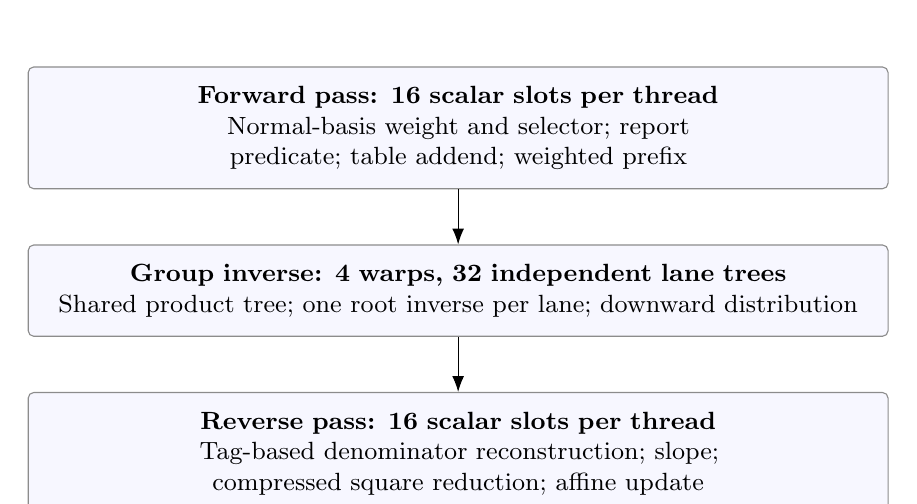
\begin{tikzpicture}[font=\small,node distance=7mm,
  box/.style={draw=black!45,rounded corners=2pt,fill=blue!3,text width=0.86\linewidth,align=center,inner sep=7pt},
  >={Latex[length=2mm]}]
\node[box] (a) {\textbf{Forward pass: 16 scalar slots per thread}\\Normal-basis weight and selector; report predicate; table addend; weighted prefix};
\node[box,below=of a] (b) {\textbf{Group inverse: 4 warps, 32 independent lane trees}\\Shared product tree; one root inverse per lane; downward distribution};
\node[box,below=of b] (c) {\textbf{Reverse pass: 16 scalar slots per thread}\\Tag-based denominator reconstruction; slope; compressed square reduction; affine update};
\draw[->] (a)--(b);\draw[->] (b)--(c);
\end{tikzpicture}
\caption{One step of the accepted two-pass kernel. Five four-warp groups fit in each 640-thread block. A lane tree shares an arithmetic inverse; it does not add independent walk points together.}
\label{fig:architecture}
\end{figure}

The receipt reports 94 registers per candidate thread and zero local bytes, compared with 116 registers and zero local bytes for the baseline. Both use 48,732 bytes of dynamic table storage. The candidate adds 12,800 bytes of static inverse scratch, with 1,024 bytes of driver-reserved shared storage. Its total is thus 62,556 bytes per block including the reservation. One block is resident per SM: 20 warps for the candidate and 16 for the baseline. These resource observations explain feasible occupancy; they do not alone establish the mechanism responsible for the measured gain.

The measured device has 188 SMs, 128 MiB of L2, an 80 MiB persisting-L2 allowance, 100 KiB of shared memory per SM, and 65,536 registers per SM. The candidate's field window exceeds the persisting allowance; the reported requested persistence covers 83,886,080 of its 98,181,120 field bytes. No assumption that all state remains in a particular cache is needed for the reported timing.

\section{Experimental methodology}\label{sec:methodology}
\subsection{Artifact and environment}
The primary evidence is the completed September 21, 2026 acceptance receipt and exported source tree~\cite{artifact}. The GPU is an NVIDIA RTX PRO 6000 Blackwell Server Edition, driver 580.95.05, with a configured 600 W power limit. The compiler identifies itself as CUDA 13.3, \code{V13.3.73}. The archive contains compiler output, device identity, binary hashes, commands, full process output, probes, and the individual timing samples.

The manuscript verification recomputed the measurement hash and checked all 119 entries of the archived source manifest. Every entry matched. An imported repository HEAD is not used as a substitute for those source hashes: the source was imported from a working tree, and the current live configuration can change independently of the archived candidate.

\subsection{Meaning of an update and the timing boundary}
The program's completed-run count is
\begin{equation}\label{eq:count}
 N=(I_{\mathrm{end}}-I_{\mathrm{start}})\,T\,B,
\end{equation}
where $T$ is the number of worker threads and $B$ the number of scalar slots per worker. The packed backend has one scalar point per slot; there is no extra factor of 32 from bitslicing. With 1,024 steps per launch and 256 launches,
\begin{align}
 N_{\mathrm{base}}&=96{,}256\cdot16\cdot1{,}024\cdot256=403{,}726{,}925{,}824,\\
 N_{\mathrm{cand}}&=120{,}320\cdot16\cdot1{,}024\cdot256=504{,}658{,}657{,}280.
\end{align}

We call these \emph{scheduled scalar-slot updates}. Every counted slot runs the complete update arithmetic, including selection and coordinate stores. However, the kernel continues to compute a slot after marking its trail finished until the launch ends and reseeding occurs. Such work is included in \cref{eq:count}. Its size is small at production settings: a slot finishes with probability $\theta_{34}$ per step (\cref{eq:dpprob}) and then idles for half a launch on average, so with 1,024 steps per launch the expected fraction of such updates is about $\theta_{34}\cdot512\approx1.3\times10^{-5}$. In benchmark mode the threshold is zero and no slot finishes. Nevertheless a scheduled update must not be interpreted as a newly useful trail point, a distinct visited state, a field multiplication, or a complete scalar multiplication $[k]P$.

The host timer starts after initialization and any checkpoint restore. It covers the launch loop, report fetching and processing, and any reseeding, and ends after a final device synchronization. Thus these are completed client-loop rates, not CUDA-event timings of an isolated kernel. Collection timing includes host report handling and file writes inside that loop. The final file close is after the printed timing boundary. Startup, table construction, initial state generation, compilation, cloud uploads, database ingestion, and an entire collision-resolution campaign are not measured by this metric.

\subsection{Confirmation protocol}
Each variant receives an excluded full-workload warmup. The harness runs five confirmation rounds and reverses the order of baseline and candidate in alternating rounds. Both variants use the same GPU allocation, 1,024 steps per launch, 256 launches, and their respective normal worker geometry. A valid sample must exit successfully, supply a final completed-run rate, match the expected update count, and report zero dropped endpoints. The paper reports the median and range of the five samples.

These timings compare complete configurations, not individual instructions. Because the candidate has 25\% more slots, the samples have different total update counts and durations. Dividing each count by its own measured duration makes a throughput comparison meaningful, while limiting attribution of the gain to any one component. Within the session the ordering is unambiguous: all five candidate samples exceed all five baseline samples, which under the null hypothesis of exchangeable samples has exact one-sided probability $1/\binom{10}{5}=1/252\approx0.004$ (Wilcoxon rank-sum). That statement concerns this session only. Five repetitions from one device session are insufficient to estimate variation across machines, drivers, days, or production workloads, and we do not report a population confidence interval.

Higher short-screening results were deliberately excluded from the headline. In particular, the 22.610829- and 22.633932-billion-update/s three-sample screens in the research notebook were used to select a candidate; the new five-sample confirmation determines the reported result. The simpler plain square-reduction candidate was selected over the combined variant, whose small screening advantage was not established independently.

\section{Results}
\subsection{Five-sample confirmation}
\begin{table}[t]
\centering
\begin{tabular}{@{}lrr@{}}
\toprule
Round & Baseline, billion/s & Candidate, billion/s\\
\midrule
1 & 20.001884 & 22.166455\\
2 & 19.867106 & 22.132776\\
3 & 19.852741 & 22.100934\\
4 & 19.841065 & 22.093414\\
5 & 19.846254 & 22.089525\\
\midrule
Median & 19.852741 & \textbf{22.100934}\\
Minimum & 19.841065 & 22.089525\\
Maximum & 20.001884 & 22.166455\\
\bottomrule
\end{tabular}
\caption{All accepted timing samples in recorded round order; one excluded warmup per variant. Every baseline sample performs 403,726,925,824 scheduled updates and every candidate sample performs 504,658,657,280.}
\label{tab:timings}
\end{table}

The ratio of medians is
\begin{equation}
 \frac{22.100934}{19.852741}=1.11324346,
\end{equation}
corresponding to an 11.3243\% improvement. Each candidate run lasts approximately 22.8 seconds under the recorded counting convention. All five candidate rates exceed 22 billion updates/s. The time series is shown in \cref{fig:rates}; the small downward trend is retained rather than hidden by selecting the fastest sample.

Post-run telemetry reports candidate SM clocks of 2,355--2,362 MHz, temperatures of 64--75 degrees Celsius, and instantaneous power readings of 544.64--584.69 W. The baseline samples report 2,400--2,415 MHz and 60--76 degrees Celsius. The candidate therefore ran about 1.6\% slower in clock terms: its median reported SM clock is 2,362 MHz against 2,400 MHz for the baseline, with both variants drawing close to the 600 W limit. Dividing each sample's rate by its own reported clock gives a ratio of medians of 1.134, a 13.4\% gain per clock cycle compared with 11.32\% in wall-clock terms. Equivalently, the candidate spends about 20.1 SM clock cycles per update and the baseline about 22.7. The wall-clock figure remains the headline because it is what a user of this power-limited device obtains. The normalized figure is indicative only: these snapshots are taken after each run and are not time-integrated traces. They do not support a joules-per-update or energy-efficiency result, and the frequencies were not fixed across the experiment. Runs with locked clocks, and runs long enough to reach thermal equilibrium, were not performed; each timed run lasts under 23 seconds while temperatures were still rising.

\begin{figure}[t]
\centering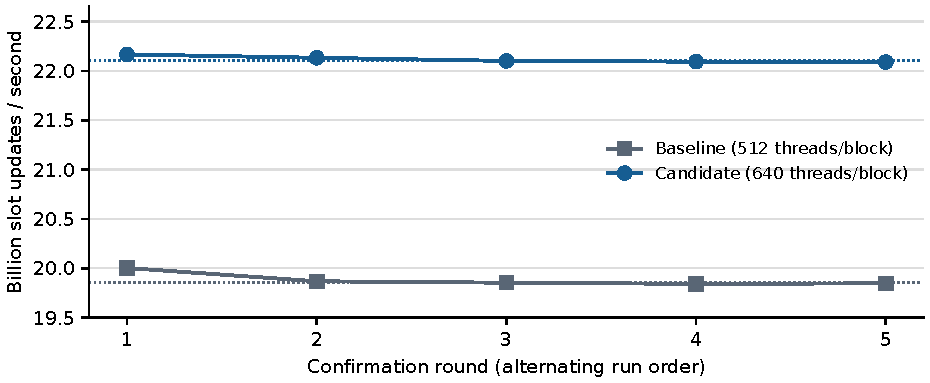
\includegraphics[width=\linewidth]{figures/confirmation-rates.pdf}
\caption{Accepted confirmation rates. Dotted lines show each variant's median. The vertical axis is deliberately restricted to show within-session drift; numerical values and full counts are provided in \cref{tab:timings}.}
\label{fig:rates}
\end{figure}

\subsection{Distinguished-point collection}
The separate DP34 candidate run completes the same 504,658,657,280 scheduled updates at 21.548499 billion/s and writes 12,387 records, totaling 396,384 bytes. It reports zero drops. Its rate is 97.5004\% of the candidate benchmark median, a descriptive difference of approximately 2.50\%. Because the collection result is one sample, this ratio is not a repeated estimate of collection overhead.

For correctness, the baseline collection run is forced to the same 120,320 workers and starting population. The two complete sorted report multisets have the same digest. This baseline geometry is deliberately different from its normal 96,256-worker benchmark geometry, so its 12.288201-billion-update/s collection rate is not used as a speedup denominator. Corpus equality requires equal initial populations; a fair throughput comparison requires appropriately specified configurations. These are different experimental requirements.

\subsection{What the measured gain does and does not isolate}\label{sec:isolate}
The baseline is the unmodified archived source tree, and the candidate is that tree with one patch. \Cref{tab:config} lists every axis on which the two measured builds differ; all other build switches, including the native carryless multiplier, the weighted prefixes, and the batch size, are identical.

\begin{table}[t]
\centering\small
\begin{tabularx}{\linewidth}{@{}>{\raggedright\arraybackslash}p{0.27\linewidth}YY@{}}
\toprule
Axis & Baseline & Candidate\\
\midrule
Inversion & One Itoh--Tsujii inverse per thread ($W=1$) & Four-warp product tree with rotated roots ($W=4$)\\
Polynomial square & Spread to 261 bits, then the general reducer & Compressed even/odd reduction, \cref{sec:square}\\
Threads per block; warps per SM & 512; 16 & 640; 20\\
Scalar slots on the device & 1,540,096 & 1,925,120\\
Kernel buffer arguments & Parameter structure & Restricted pointers\\
Live metadata per slot & 32-bit finished flag; 64-bit history & One byte; three 16-bit tags\\
Paired-product instruction interleaving & Enabled & Disabled\\
Registers per thread & 116 & 94\\
Shared inverse scratch per block & None & 12,800 bytes\\
Field bytes; persisting-L2 coverage & 78,544,896; all & 98,181,120; 83,886,080\\
\bottomrule
\end{tabularx}
\caption{Every difference between the two measured builds, taken from the archived patch and from the configuration banner that each run prints. Forward selection pipelining is disabled in both.}
\label{tab:config}
\end{table}

The confirmation compares only the two ends of this list, so it cannot attribute the gain. The multiplication-count reduction in \cref{eq:cost} is 4.41\%, smaller than the measured 11.32\%. The screening receipts give a partial attribution, because the candidate was built up in stages and every stage was timed against a baseline in the same session (\cref{tab:ladder}).

\begin{table}[t]
\centering\small
\begin{tabularx}{\linewidth}{@{}Yrrr@{}}
\toprule
Configuration (cumulative) & Arm, billion/s & Baseline, billion/s & Gain\\
\midrule
Compact metadata, 640 threads, no interleaving & 20.231 & 19.980 & $+1.26\%$\\
\quad plus restricted pointers & 20.564 & 20.095 & $+2.33\%$\\
\quad plus rotated four-warp inversion & 21.756 & 20.087 & $+8.31\%$\\
\quad plus shorter spread before the general reducer & 21.841 & 19.791 & $+10.36\%$\\
\quad with compressed square reduction instead & 22.611 & 20.071 & $+12.66\%$\\
\midrule
Same configuration, five-sample confirmation & 22.101 & 19.853 & $+11.32\%$\\
\bottomrule
\end{tabularx}
\caption{Screening sequence. Each row is the median of three samples against the median of three baseline samples from the same session; the last row repeats \cref{tab:timings}. Sessions differ in clocks and temperature, so gains are comparable across rows only approximately.}
\label{tab:ladder}
\end{table}

Three observations follow. First, the inversion tree at the wider geometry is the largest step, about six percentage points. It depends on the geometry and on root placement: the same tree gave $+3.67\%$ at 512 threads, and an earlier unrotated four-warp tree on the unmodified 512-thread kernel was \emph{slower} than its baseline by $3.06\%$. Second, restricted pointers help only together with the wider block; at 512 threads with interleaving enabled they measured $-0.30\%$. Third, the compressed square adds three to four percentage points over the preceding configurations, and about two over the shorter spread alone. This step is larger than an operation count suggests. The root inverse converts to the normal basis, where squaring is a permutation, so the polynomial square runs only once per update, beside roughly five multiplications. The shorter routine probably also relieves register or scheduling pressure in the reverse pass; an isolated microbenchmark would be needed to confirm that.

This sequence is not a controlled factorial ablation. The stages were measured in different sessions, with three samples each, and no stage removes a single component from the final candidate. A controlled study would disable one row of \cref{tab:config} at a time within one alternating session, and would add an isolated microbenchmark of the two squaring routines. That study has not been run. The notebook also records unsuccessful alternatives, including binary-GCD inversion, larger per-thread batches, wider blocks, alternate shared-table layouts, and earlier collective schemes. An earlier primitive-probe include-path error was subsequently corrected; only the final receipt's intended-header probes and confirmation samples are used for acceptance here.

\section{Correctness evidence and practical limits}
\subsection{Evidence retained with the result}
\begin{table}[t]
\centering\small
\begin{tabularx}{\linewidth}{@{}>{\raggedright\arraybackslash}p{0.27\linewidth}Y>{\raggedright\arraybackslash}p{0.17\linewidth}@{}}
\toprule
Check & Recorded coverage & Outcome\\
\midrule
Source integrity & 119 archived files; measurement digest & All matched locally\\
Polynomial square identity & 131 basis inputs, two edge cases, 10,000 random values & Passed locally\\
GPU field probes & 1,133 squares, 1,133 inverses, 6,798 Frobenius maps & Receipt passed\\
GPU group inverse & 1,024 inputs for each $W=2,4,8,16$; zeros and consecutive calls & Receipt passed\\
GPU metadata & 1,025 lanes; byte flags; 200 history updates/lane & Receipt passed\\
Independent trail replay & 300 reports with endpoint and length equality & Receipt passed\\
Complete replay corpus & 32,688 records at matched population & Digests equal\\
DP34 collection corpus & 12,387 records; 396,384 bytes & Digests equal\\
Checkpoint continuation & Baseline $\to$ candidate and reverse & Receipt passed\\
Compute Sanitizer & Device/runtime support unavailable & Not passed\\
Inherited \code{test-clmad} & Source/guard expectation failures remain & Not fully green\\
\bottomrule
\end{tabularx}
\caption{Evidence classes. ``Receipt passed'' denotes a recorded GPU check, not a new run performed while preparing this manuscript. The algebraic identity check covers the full linear map; the other finite checks have their stated coverage.}
\label{tab:validation}
\end{table}

The independent field probes compare against \code{Ref<CfgF131>}, rather than merely comparing the candidate with a second use of the same optimized routine. The final receipt also includes the selected collective helper hash and probes the composed arithmetic implementation. The full replay comparison uses 65,536 starting scalar walks, six launches, and 16 steps per launch with reporting threshold 50. Equality is established for the complete sorted multiset of 32,688 persisted records, not just a sampled prefix.

Checkpoint tests split the same workload into three launches in one build and three in the other, then compare against uninterrupted execution. This tests observable continuation across the two memory representations. It does not establish compatibility with every future walk, campaign, or checkpoint format.

The final collection corpora themselves are summarized by retained hashes and counts in the receipt; the manuscript package does not claim to include the original binary corpus files. Reproducing those digests requires rerunning the documented client with the matching seeds and population. Similarly, the measured executable is identified by hash but is not claimed to have been reconstructed byte for byte by the local manuscript build.

\subsection{Exceptional affine additions}\label{sec:exceptional}
The fast path implements \cref{eq:affine} without complete handling of $d=0$, and the host table reference intentionally uses the corresponding raw addition. Agreement between those two paths therefore does not establish correct group behavior for an exceptional input. A zero denominator invalidates the affected thread's local prefix chain: the batch product is zero, the returned inverse is zero, and all 16 slots of that thread receive $\lambda=0$. Cross-warp zero isolation protects other batches but does not resolve that case.

The exceptional set is small and explicit. The denominator vanishes exactly when the current point and the selected addend share an $x$ coordinate, that is when $R=\pm\sigma^{k}(T_h)$ for the selected $(h,k)$. At most $2\cdot8\cdot131=2{,}096$ subgroup points have this form. Under the usual heuristic that visited points are uniform in the subgroup, the probability per step is at most
\begin{equation}
 \frac{2{,}096}{\ell}\approx3.1\times10^{-36},
\end{equation}
and the expected number of occurrences over an entire search of $2^{60.8}$ steps is about $6\times10^{-18}$. This bound is heuristic. It assumes that the public table seed does not correlate the table orbits with the starting points, and it is not a proven exclusion condition.

Detection needs no additional field arithmetic. The per-thread batch product is zero exactly when some $d_i=0$ in that batch, and the collective helper already evaluates that zero test once per thread and step in order to isolate other warps. A complete policy is therefore to mark all 16 slots of a thread as finished whenever its returned inverse is zero, so that the ordinary reseed path replaces them. Discarding 16 trails with probability near $10^{-35}$ per step has no measurable effect on useful work. This policy is not implemented in the archived candidate and its cost was not timed; the archived timing and replay evidence establish the tested ordinary-domain behavior only.

\subsection{Collision quality and useful work}
The familiar square-root collision estimate requires an appropriate model of the actual transition system. The estimates in \cref{sec:history} bound two of the open effects under a uniform model: about $0.1\%$ of merges fail to coalesce because of the history rule, and on the order of $1\%$ of DP34 trails enter a six-step fruitless cycle, which makes the restart limit a first-order parameter of a production run. Neither estimate has been measured, and the nonuniform branch index and the projection to an orbit key are not covered by them. The acceptance receipt does not test the source's claim that merged trails resynchronize. Equal deterministic output between two implementations of the same walk is a strong regression check, but it does not validate that walk's random-map model.

A useful next evaluation would measure, on tractable public instances, the distribution of collision times, the proportion of useful independent collisions, trail coalescence after histories differ, and the fraction of trails that reach the restart limit as a function of that limit. The last two measurements test the two estimates above directly. Such a study must preserve the selector and correction rule or explicitly account for any difference. It would supply information that update throughput alone cannot provide. Consequently we do not convert 22.100934 billion updates/s into a projected challenge completion time or a claimed security-bit reduction.

\subsection{Statistical and system limits}
The experiment uses one GPU allocation and one toolchain/driver combination. Thermal drift is visible and the device is power-limited, so the two variants ran at different clocks; collection has one repetition; the attribution in \cref{tab:ladder} rests on three-sample screens from separate sessions; no locked-clock run, energy integral, multi-device variance, or long-duration sustained-load distribution is available. Compute Sanitizer was unavailable on the device/runtime, and the inherited \code{test-clmad} suite has unresolved source-shape and architecture-guard expectations. These facts remain explicit even though the selected independent functional probes passed.

The repository also contains cloud persistence and worker-launch evidence. That evidence has a different scope and is excluded from the headline result. No fleet scaling factor, S3/RDS throughput guarantee, or completed challenge computation follows from this single-device acceptance receipt.

\section{Reproducibility and artifact availability}
The paper's evidence boundary is the archived directory
\begin{center}
\path{ecc2k130/research/candidates/goal22/}.
\end{center}
The accompanying manuscript package includes the raw measurement receipt, acceptance record, source manifest, derived statistics, and a script that checks the local archive and regenerates the performance figure. The complete source tree remains in that archived directory. This draft does not assert a publicly accessible archival release or invent a repository commit for uncommitted source.

On a compatible CUDA environment, build the archive's own target:
\begin{lstlisting}
cd ecc2k130/research/candidates/goal22
make gpu-goal22
./ecc2k130 --curve 131 --packed --bench \
  --steps 1024 --launches 256 --verify 0
\end{lstlisting}
This single invocation is a workload command, not the full acceptance protocol. Reproduction must restore the recorded compiler and GPU target, run the independent probes, exclude warmups, alternate the control and candidate over five rounds, retain final counts, and separately repeat collection. The manifest contains the complete 33-token build command and binary identity. The original confirmation also records the baseline build and its output in the measurement receipt.

Before public submission, an immutable source-and-evidence deposit would make these local artifact references independently accessible. The unresolved exceptional-input and collision-quality questions should accompany that deposit, so that a reader can reproduce both the strengths and the limits of the result.

\section{Conclusion}
The accepted ECC2K-130 table-walk configuration reaches a five-sample median of 22.100934 billion scheduled scalar-slot updates/s on one RTX PRO 6000 Blackwell GPU, improving on its same-run local baseline by 11.32\%. A separate collection run reaches 21.548499 billion updates/s with zero reported drops and a matching complete report corpus. The implementation combines native carryless multiplication, polynomial state, four-warp batch inversion, compact metadata, and a square-and-reduce circuit that exploits the even-coefficient structure of binary squaring.

The most transferable result is the joint treatment of arithmetic and GPU scheduling, together with an explicit link from performance claims to immutable evidence. The screening sequence attributes the largest share of the gain to the rotated inversion tree at the wider geometry and three to four percentage points to the square, without a controlled ablation. The selector is defined on every reachable point, and exceptional additions are both negligible in probability and detectable from the existing zero test. The next step toward a complete state-of-the-art collision-search claim is to implement that policy, to measure coalescence and the six-step cycle rate of the history-dependent walk on tractable instances, and then to measure the resulting useful work with a restart limit under sustained, locked-clock conditions.

\bibliographystyle{plain}
\bibliography{references}

\clearpage
\appendix
\section{Artifact identities and implementation map}
\small
\begin{tabularx}{\linewidth}{@{}lY@{}}
\toprule
Object & SHA-256\\
\midrule
Measurement receipt & \hashval{840b6071d202393a958b00317be58d90f}{b2a9367363659d18daaaebba2dc4d82}\\
Candidate executable & \hashval{da24894bdef26c638b243790a3bf4cf1}{66feecac27221cd8c035191dc20d9e9a}\\
Baseline executable & \hashval{b62f1c6162164dcea69c7478525f8a0a}{f65bb295420ce919da9830f4fc1a0500}\\
Replay corpus (sorted) & \hashval{db31c5c36206192fe8fda4cba58152e4}{6620d2ffe5e4d22605e7f7d34909162e}\\
DP34 corpus (sorted) & \hashval{334b830fc6d3bf5801013203010bb030}{baddfdc5950f11c8a881a5c95ff9c092}\\
\bottomrule
\end{tabularx}
\normalsize
\medskip
The recorded GPU UUID is \path{GPU-080ac0e6-6dbe-3064-5ce3-7fe34abd5193}. The archived candidate name, hashes, and source manifest identify this study even if the live build profile changes.

\begin{table}[H]
\centering\small
\begin{tabularx}{\linewidth}{@{}>{\raggedright\arraybackslash}p{0.32\linewidth}Y@{}}
\toprule
Paper component & Archived implementation\\
\midrule
Curve and field constants & \path{generated/eccF131.h}\\
Reference table and raw update & \path{include/ref.h}, \code{TableWalk<Cfg>}\\
Phase, pivot, cycle tags & \path{include/tablewalk.h}\\
Device selection and addends & \path{include/packedtablewalk.cuh}\\
Algorithm~\ref{alg:batch} forward/reverse passes & \path{include/packedkernels.cuh}, \code{walk}\\
Four-warp inverse & \path{include/collective_inverse.cuh},\newline \code{goal22CollectiveInverse<4>}\\
Compressed square reduction & \path{research/gen_square_reduce.py}; \path{include/square_reduce.h}\\
Packed state and metadata & \path{include/packedcompactstate.cuh}; \path{include/compact_metadata.cuh}\\
Timer and update accounting & \path{src/main.cu}, completed-run output\\
\bottomrule
\end{tabularx}
\caption{Mapping between manuscript algorithms and the frozen source. All paths in this table are relative to the archived candidate directory.}
\end{table}

\section{Zero handling and product-tree invariant}
For nonzero leaves $d_0,\ldots,d_{W-1}$, each upward tree node stores the product of its descendant leaves. If a node with children $L,R$ holds $(LR)^{-1}$, its child inverses are $R(LR)^{-1}=L^{-1}$ and $L(LR)^{-1}=R^{-1}$. The downward pass therefore returns each original leaf inverse. Replacing a zero leaf by one before this construction keeps the product invertible; restoring zero at that output implements the helper's explicit convention $\operatorname{inv}(0)=0$.

The logical warp permutation is bijective within each barrier group and leaves lane positions unchanged. Each group consequently runs 32 separate product trees, and no operand crosses a group boundary. This algebraic invariant explains the returned values. Race freedom and barrier participation still rely on the actual synchronization implementation and are supported by finite device tests, with the sanitizer limitation reported in \cref{tab:validation}.

\end{document}
